\chapter{Números/Relações (3º Bimestre)}

\section{Equações de 1º grau e funções linerares}

\subsection*{Resumo}

Se $a$, $b$ são números constantes tal que $a \neq 0$, uma equação linear se
escreve $a x + b = 0$ onde $x$ é a incógnita. A única solução desta equação é $x
= - b / a$.

Se $a, b$ são números constantes, a função $f(x) = a x + b$ é uma função linear.
O gráfico de uma função $f(x) = a x + b$ é o conjunto de pontos de coordenadas
$(x, y)$ onde $y = a x + b$. O gráfico de $f$ intersecta o eixo vertical $y$
no ponto $P_0 = (x_0, y_0)$ onde $x_0 = 0$ e $y_0 = b$. Se $a = 0$ a funçã $f$ é
constante com valor $b$ e seu gráfico é uma reta paralela ao eixo horizontal $x$
de equação $y = b$. Se $a \neq 0$ e $P = (x, y)$ é um ponto do gráfico ($x \neq
x_0$) e $y - y_0 = a {(x - x_0)}$ e então a direção da reta $(P_0P)$ é dado por
$\frac{1}{{(x - x_0)}} ({x - x_0}, {y - y_0}) = {(1,a)}$. A inversa, os pontos
$P = (x, y)$ da reta passando por $P_0$ e de direção $(1, a)$ satisfazem
$({x - x_0}, {y - y_0}) = k {(1,a)}$ para algum $k$ e então
$k = x - x_0 = \frac{y - y_0}{a}$ temos $y = a {(x + x_0)} + y_0 = a x + b$.

Finalmente, o gráfico de $f$ é a reta passando por $(0, b)$ e de direção $(1,
a)$. Se $a \neq 0$, o gráfico de $f$ intersecta a o eixo $x$ verticalmente no
ponto $P_1 = (x_1, y_1)$ onde $y_1 = 0$ e $x_1 = -\frac{b}{a}$ é a solução da
equação linear $f(x) = ax + b = 0$.  Então, o gráfico de $f$ é a reta
$(P_0P_1)$.

O ângulo da reta é dado pelo parâmetro $a$. Se $a = 0$, a reta é paralela ao
exio horizontal $x$, a função é constante. Se $a < 0$, quando o valor de $x$
aumenta em uma unidade, o valor de $y$ diminue em $|a|$ unidades, a função é
decrescente.
Se $a < 0$, quando o valor de $x$ aumenta em uma unidade, o valor de $y$ aumenta
em $a$ unidade, a função é crescente. Duas funções lineares com o mesmo
coeficiente $a$ são paralelas.

\subsection*{Exemplo}

Esses são gráficos de três funções linerares que são retas. A reta verde de
equação $y = 20$ é paralela ao eixo $x$ ($a = 0$) e passa pelo ponto $(0,20)$. A
reta azul de equação $y = 2 x + 10$ é crescente ($2 > 0$) e intersecta o eixo
$x$ em $x = -\frac{10}{2} = -5$ e o eixo $y$ em $y = 10$. A reta vermelha de
equação $y = -6x + 15$ é decrescente ($-6 < 0$) e intersecta o eixo $x$ em $x =
-\frac{15}{-6} = 2.5$ e o eixo $y$ em $y = 15$. O ângulo da reta vermelha ($|a|
= 6$) é maior que o ângulo da reta azul ($|a| = 2$) e portanto a primeira
decresce mais rápido que a segunda cresce.

\begin{center}
  \begin{tikzpicture}[domain=-10:10, xscale=.5, yscale=0.05]
    \draw[->] (-10.5,0) -- (10.5,0) node[right] {$x$};
    \draw[->] (0,-60.5) -- (0,60.5) node[above] {$y$};
    \draw[color=blue]    plot (\x,2*\x+10)       node[left] {$y=2x+10$};
    \draw[color=red]   plot (\x,{-6*\x + 15})    node[left] {$y = -6x+15$};
    \draw[color=green] plot (\x,{20}) node[left] {$y = 20$};
    \foreach \x in {-10,-5,5,10}
      \draw (\x,-1) --(\x,1) node[above] {$\x$};
    \foreach \y in {-40,-20,20,40}
      \draw (-.2, \y) --(.2, \y) node[right] {$\y$};
  \end{tikzpicture}
\end{center}

\subsection*{Exercício 1}

Encontre a solução das seguintes equações lineares:

\begin{enumerate}
\item $2x+3 = 0$
\item $2x-10 = 0$
\item $-3x-9 = 0$
\end{enumerate}

\subsection*{Exercício 2}

Rascunhe o gráfico das funções lineares
$f(x) = 2x+1$, $g(x) = 2x-10$, $h(x)=-3x-12$. Deduza, graficamente, as soluções
das equações anteriores. O que podemos dizer sobre las retas $f$ e $g$? O que
podemos dizer sobre o ângulo da reta $h$?

\subsection*{Exercício 3}

Identificar os gráficos de
$y = 10$, $y=-2x+15$, $y=-2x+5$, $y=2x+10$, $y=3x+10$
e $y=\frac{x^2}{10} + 10$ na figura abaixo:

\begin{center}
  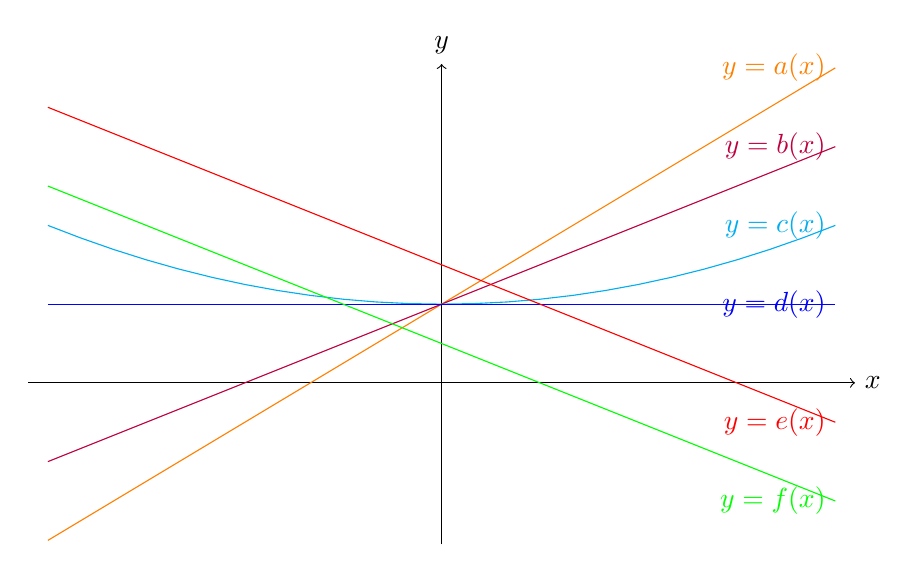
\begin{tikzpicture}[domain=-10:10, xscale=.5, yscale=0.1]
    \draw[->] (-10.5,0) -- (10.5,0) node[right] {$x$};
    \draw[->] (0,-20.5) -- (0,40.5) node[above] {$y$};
    \draw[color=orange] plot (\x,{3*\x + 10}) node[left] {$y=a(x)$};
    \draw[color=purple] plot (\x,{2*\x + 10}) node[left] {$y=b(x)$};
    \draw[color=cyan] plot (\x,{\x*\x/10 + 10}) node[left] {$y=c(x)$};
    \draw[color=blue]    plot (\x,10)       node[left] {$y=d(x)$};
    \draw[color=red]   plot (\x,{-2*\x + 15})    node[left] {$y=e(x)$};
    \draw[color=green] plot (\x,{-2*\x + 5}) node[left] {$y=f(x)$};
  \end{tikzpicture}
\end{center}

\subsection*{Exercício 4}

João vende uma caixa de $6$ ovos por $\text{R\$}2,00$ e a comida das galinhas
lhe custa $\text{R\$}31,00$ cada dia. Expresse o dinheiro que João ganha cada
dia que trabalha em função do número de caixas $N$ que vende. Rascunhe o gráfico
para $0 \leq N \leq 20$ e deduza o mínimo de caixas que precisa vender para não
sair no prejuízo. Compare com a solução da equação linear $2x - 31 = 0$.

\section{Sistemas lineares de duas incógnitas}

\subsection*{Resumo}

Um sistema de equações (lineares) com duas incógnitas é um conjunto finito de
equações $a x + b y = c$ onde $x$, $y$ são incógnita e $a$, $b$. $b$ constantes.
Um sistema de $n$ equações pode ser escrito

$\left\{
\begin{aligned}
  a_1 x + b_1 y = c_1 \\
  a_2 x + b_2 y = c_2 \\
  \ldots \\
  a_n x + b_n y = c_n
\end{aligned}\right.$

Podemos efetuar várias operações para resolver o sistema. As operações devem ser
inversíveis para conservar a equivalência com o sistema original.

\begin{enumerate}
\item Tomar a soma de duas equações para obter uma terceira equação:
${(a_1+a_2)} x + {(b_1+b_2)} y = c_1 + c_2$.
\item Ou a subtração de duas equações: ${(a_1-a_2)} x + {(b_1-b_2)} y = c_1 - c_2$.
\item Multiplicar/Dividir uma equação por uma constante $k$:
  $k a_1 x + k b_1 y = k c_1$.
\item Realizar uma substituição. Por exemplo, se $a_1 = 1$,
  $x = c_1 - b_1 y$ e fazendo esta substituição na segunda equação, obtemos
  $a_2 c_1 + (b_2 - a_2 b_1) y  = c_2$.
\end{enumerate}

Supondo que o sistema possua apenas uma equação $a x + b y = c$.
Se $a = b = c = 0$, todos os $(x,y) \in {\mathbb R}^2$ são soluções.
Se $a = b = 0$ e $c \neq 0$ não existe solução. $b \neq 0$, obtemos a
equação $y = -\frac{a}{c}x +\frac{c}{b}$ então existe infinitas soluções
$(x, y)$ para cada $x \in {\mathbb R}$. Da mesma maneira, se $a \neq 0$, existe
infinitas soluções $({-\frac{b}{a}y+\frac{c}{a}}, y)$
para cada $y \in {\mathbb R}$.

Agora, considerando as equações $ax+by=k$ e $cx+dy=l$. Multiplicando
a primeira equação por $c$ e a segunda por $a$, obtemos

$\left\{
\begin{aligned}
  ca x + cb y = ck \\
  ac x + ad y = al \\
\end{aligned}\right.$

e se tomarmos o resto das duas obtemos
${(ad - bc)} y = ck - al$. Então, se o determinante
$\Delta = ad - bc$ não é zero obtemos $y = \frac{al - ck}{\Delta}$. Da
mesma maneira, obtemos $x = \frac{dk - bl}{\Delta}$ e portanto o sistema
possue uma solução $(x, y)$. Se $\Delta = 0$, $ad = bc$ e
$al = a{(cx+dy)} = acx + ady = acx+bcy = c{(ax+by)} = ck$ e da mesma maneira
$bl = dk$. Então se $a \neq 0$, as soluções são da equação,
$ax + by = k$ se $l = -\frac{ck}{a}$ e se não existe solução. Se $b \neq 0$,
as soluções são da equação $ax + by = k$ se $l = -\frac{dk}{b}$
e se não existe solução. Se $a = b = 0$, as soluções são da equação
$cx + dy = l$ se $k = 0$ e se não existe solução.

Podemos aplicar esses métodos para resolver um sistema de $n \geq 3$ equações.
Em geral, duas equações determinam uma solução única $(x,y)$ e portanto um
sistema de $n \geq 3$ equações não possui solução se essas soluções não são
compatíveis.

\subsection*{Exemplo}

\begin{enumerate}
\item
$\left\{\begin{aligned}
  4x + 3y = 0 \\
  z = x + y
\end{aligned}\right.$ não é um sistema de duas equações (possui três variáveis).

\item
$\left\{\begin{aligned}
  x^2 + 2y = 1 \\
  x + \sqrt{y} = -2
\end{aligned}\right.$ não é um sistema linear (contem $x^2, \sqrt{y}$)

\item
$\left\{
\begin{aligned}
  4x + 3y = 2x - 7 \\
  3x = 2x + 3y
\end{aligned}\right.$ é um sistema de duas equações, equivale a forma
simplificada
$\left\{
\begin{aligned}
  2x+3y = -7 \\
  x -4y = 0
\end{aligned}\right.$
\item $2x + y = 1$ possui infinitas soluções.
  $\{ {(x, y)} : x \in \mathbb R, y = 1 - 2x \}$
\item $5x = 2$ possui infinitas soluções.
  $\{ {(\frac{2}{5}, y)} : y \in {\mathbb R} \}$
\item  Para resolver $\left\{
\begin{aligned}
  2x+3y = -7 \\
  x -4y = 0
\end{aligned}\right.$ podemos fazer a substituição $x = 4y$ na primeira
equação: $8y + 3y = -7$ equivale
$y = -\frac{7}{11}$ e $x = 4y = -\frac{28}{11}$.
\item  Para resolver $\left\{
\begin{aligned}
  2x+3y = -7 \\
  x -4y = 0
\end{aligned}\right.$ podemos multiplicar a segunda equação por 2:
$2x - 8y = 0$ e tomar o resto em relação a primeira:
$-7 - 0 = {(2x + 3y)} - {(2x-8y)} = 11y$. Então $y = -\frac{7}{11}$ e
$x = 4y = -\frac{28}{11}$.
\item  Para resolver $\left\{
\begin{aligned}
  2x+3y = -7 \\
  x -4y = 0
\end{aligned}\right.$ podemos calcular o determinante
$\Delta = 2 \times -4 - 3 \times 1 = -11$ e utilizar as fórmulas
$x = \frac{-4 \times -7 - 2 \times 0}{-11} = -\frac{28}{11}$ e
$y = \frac{2 \times 0 - 1 \times -7}{-11} = -\frac{7}{11}$.
\item  O determinante de $\left\{
\begin{aligned}
  -21x+6y = 3 \\
  7x-2y = 2
\end{aligned}\right.$ é $\Delta = -21 \times -2 - 6 \times 7 = 0$. Se
multiplicamos a primeira por $-\frac{1}{3}$, obtemos $7x-2y=-1$ então
não é compatível com a segunda equação $7x-2y = 2$ e o sistema não possui
solução.
\item O sistema de três equaçõesc $\left\{
\begin{aligned}
  -4x-6y = 14 \\
  x -4y = 0 \\
  2x+3y = -7
\end{aligned}\right.$ a primeira equações equivale a terceira e
portanto reduzimos o sistema para duas equações $\left\{\begin{aligned}
  2x+3y = -7 \\
  x -4y = 0
\end{aligned}\right.$ a solução é $y = -\frac{7}{11}$ e
$x = -\frac{28}{7}$.
\item $y = -\frac{7}{11}$ e $x = -\frac{28}{11}$ é a única solução das duas
últmas equações de $\left\{
\begin{aligned}
  22y = -14 \\
  x -4y = 0 \\
  2x+3y = -7
\end{aligned}\right.$ e $22 \times -\frac{7}{11} = -14$ portanto também é a
solução do sistema de três equações.

\item $y = -\frac{7}{11}$ e $x = -\frac{28}{11}$ é a única solução das duas
últimas equações de $\left\{
\begin{aligned}
  11x = 2 \\
  x -4y = 0 \\
  2x+3y = -7
\end{aligned}\right.$ mas
$11 \times -\frac{28}{11} = -28 \neq 2$ portanto o sistema de três equações não
possui solução.

\end{enumerate}

\subsection*{Exercício 5}

Resolver o sistema seguintes com duas incógnitas $x$ e $y$:

\begin{enumerate}
\item $x + 2 - 9y = 8 - 3y + 2x$
\item $\left\{\begin{aligned}
  3x + 2y = 8 \\
  y - 7 = 2y + 3
\end{aligned}\right.$
\item $\left\{\begin{aligned}
   7x  - 8y = 4 \\
  -3x + 5y = 7
\end{aligned}\right.$

\item $\left\{\begin{aligned}
   21x  - 14y = 4 \\
  -3x + 2y = 7
\end{aligned}\right.$

\item $\left\{\begin{aligned}
   3x-2y=2+6y \\
  4x-8y=4-2x+8y
\end{aligned}\right.$

\item $\left\{\begin{aligned}
   2x-7y=9 \\
  2x=2-9y \\
  4x-10y-9=9+4y
\end{aligned}\right.$

\item $\left\{\begin{aligned}
   7x  - 8y = 4 \\
  -3x + 5y = 7 \\
  x - y = 0
\end{aligned}\right.$

\end{enumerate}

\subsection*{Exercício 6}

Determinar o determinante desses sistemas e encontra as soluções.

\begin{enumerate}
\item $\left\{\begin{aligned}
  3x+y=-2 \\
  27x-9y=0
\end{aligned}\right.$
\item $\left\{\begin{aligned} 3x+y=-2\\ 27x+9y=0\end{aligned}\right.$
\item $\left\{\begin{aligned} 8x+y=64\\ \frac{x}{2}+\frac{y}{16}=4\end{aligned}\right.$
\end{enumerate}

\section{Interpretação gráfica}

\subsection*{Resumo}

Como vimos no capítulo anterior,
se $a,b \neq 0$, as soluções da equação $ax+by=c$ no plano
${\mathbb R}^2$ são os pontos da reta passando por $(0, -\frac{c}{b})$ e
$(-\frac{c}{a}, 0)$. Se $a = 0$ e $b \neq 0$, a reta passando por
$(0, -\frac{c}{b})$ e paralela ao eixo $y$. Se $a = 0$ e $b \neq 0$, é a reta
passando por $(-\frac{c}{a}, 0)$ e paralela ao eixo $x$. Finalmente, se
$a = b = 0$ é todo o plano (se $c = 0$) ou o conjunto vazio ($c \neq 0$).

Para um sistema de duas equações, tomando a intersecção dos dois conjuntos.
Em geral (se nenhum é vazio ou todo o plano) temos duas retas. Se as equações
são incompatíveis, as retas são paralelas e a intersecção é vazia.
de outra maneira, existe uma única solução que é a intersecção das duas retas.

Para um sistema de $n \geq 3$ equações, em geral temos três $n$ retas que
possuem com sorte uma intersecção comum.

\subsection*{Exemplo}

Podemos ver as retas representando a solução das equações
$x=-4$, $y=-5$, $x-2y=6$, $x-2y=0$, $5x-4y=0$. As retas $x=-4$ e $y = -5$ são
paralela aos eixos. As retas $x - 2y$ e $x - 2y = 6$ são paralelas e
portanto o sistema $\left\{\begin{aligned}
   x-2y=0 \\
  x-2y=6
\end{aligned}\right.$ não possui solução. As retas $5x - 4y = 0$ e
$x - 2y = 6$ se interceptam em $(-4, -5)$ e portanto a única solução do sistema
é $\left\{\begin{aligned}
   5x-4y=0 \\
  x-2y=6
\end{aligned}\right.$

\begin{center}
  \begin{tikzpicture}[domain=-10:10, xscale=.5, yscale=.5]
    \draw[->] (-11,0) -- (11,0) node[right] {$x$};
    \draw[->] (0,-11) -- (0,11) node[above] {$y$};
    \draw[color=blue] plot (\x,\x/2-3) node[left] {$x - 2y = 6$};
    \draw[color=red] (-10,-5)--(8,-5) node[above] {$y = -5$};
    \draw[color=green] (-4,-10)--(-4,10) node[left] {$x = -4$};
    \draw[color=orange] plot (\x,\x/2) node[left] {$x - 2y = 0$};
    \draw[color=purple] plot (\x,5*\x/4) node[left] {$5x - 4y = 0$};

    \foreach \x in {-10,-5,5,10}
      \draw (\x,-.1) --(\x,.1) node[above] {$\x$};
    \foreach \y in {-10,-5,5,10}
      \draw (-.1,\y) --(.1,\y) node[left] {$\y$};
  \end{tikzpicture}
\end{center}

\subsection*{Exercício 7}

Rascunhar o gráfico das equações $3x-y=5$ e $2x-3y=7$. Deduzir a solução do
sistema $\left\{\begin{aligned}
   3x-y=5 \\
  2x-3y=7
\end{aligned}\right.$

\subsection*{Exercício 8 (problema)}

João vende $1$ litro de leite a $\text{R\$}2,50$ e a comida de suas vacas custa-lhe
$\text{R\$}4,00$ mais $\text{R\$}0,50$ para cada litro.
Represente o custo de $x$ litros e da comida das vavas
no mesmo gráfico, para $0 \leq x \leq 5$. Deduza o mínimo de leite que deve ser
vendido para que João não tenha um prejuízo.

\section{Solução dos exercicios}

\subsection*{Exercício 1}

\begin{enumerate}
\item $x = -\frac{3}{2}$
\item $x = 5$
\item $x = -3$
\end{enumerate}

\subsection*{Exercício 2}

As soluções são dadas pelas intersecções das retas com o eixo $x$.
$x_f = -\frac{1}{2}, x_g = 5, x_h = -4$. A reta de $f$ e $g$ são paralelas
pois as equações possuem o mesmo coeficiente angular $a = 2$. $-3 < 0$ e ${|-3|} < 2$
então $h$ decresce e seu ângulo é mais importante que o das outras retas.

\begin{center}
  \begin{tikzpicture}[domain=-10:10, xscale=.5, yscale=0.1]
    \draw[->] (-10.5,0) -- (10.5,0) node[right] {$x$};
    \draw[->] (0,-40.5) -- (0,40.5) node[above] {$y$};
    \draw[color=blue]    plot (\x,2*\x+1)       node[left] {$y=f(x)$};
    \draw[color=red]   plot (\x,{2*\x -10})    node[left] {$y=g(x)$};
    \draw[color=green] plot (\x,{-3*\x - 12}) node[left] {$y=h(x)$};
    \foreach \x in {-10,...,10}
      \draw (\x,-1) --(\x,1) node[above] {$\x$};
    \foreach \y in {-40,-20,20,40}
      \draw (-.2, \y) --(.2, \y) node[right] {$\y$};
  \end{tikzpicture}
\end{center}

\subsection*{Exercício 3}

O gráfico de $c(x)=\frac{x^2}{10} + 10$ não é uma reta.
$d(x) = 10$ é constante e corresponde a reta paralela ao exio $x$.
A reta $a(x) = 3x+10$ e $b(x) = 2x+10$ intersectam o eixo $y$ em
$y = 10$ e a primeira cresce mais rápido que a segunda porque $3 > 2$.
As retas paralelas são dadas por $e(x) = -2x+15$ e $f(x) = -2x+5$ e as
funções são decrescente (possuem o mesmo $a=-2 < 0$). A primeira reta está
acima porque $15 > 5$.

\subsection*{Exercício 4 (problema)}

O lucro é $B(N) = 2N - 31$ reais.
Os pontos para $0 \leq N \leq 20$ estão
sobre a reta da equação $y = 2x - 31$ e o lucro é positivo para
$N \geq 16$. A solução da equação $2x - 31 = 0$ é
$x = \frac{31}{2} = 15.5$ e o mínimo de caixas é o menor inteiro maior que
$\geq 15.5$.

\begin{center}
  \begin{tikzpicture}[domain=-10:10, xscale=.5, yscale=.25]
    \draw[->] (0,0) -- (22,0) node[right] {$N$ (cajas)};
    \draw[->] (0,-35) -- (0,17) node[above] {$B(N)$ (R\$)};
    \foreach \N in {0,...,20}
      \draw (\N, 2*\N - 31) circle(.5);
    \foreach \N in {0,5,10,15,20}
      \draw (\N,-1) --(\N,1) node[above] {$\N$};
    \foreach \B in {-35,-30,-25,-20,-15,-10,-5,5,10,15}
      \draw (-.2, \B) --(.2, \B) node[right] {$\B$};
  \end{tikzpicture}
\end{center}

\subsection*{Exercício 5}

\begin{enumerate}
\item A equação é simplificada em $y = \frac{x}{6} - 1$. Possui infinitas
  soluções ${(x, \frac{x}{6} - 1)}$
\item $\left\{\begin{aligned}
  3x + 2y = 8 \\
  y - 7 = 2y + 3
\end{aligned}\right.$ A segunda equação é simplificada em $y = -10$.
  Então, da primeira temos $3x - 20 = 8$ e $x = \frac{28}{3}$.
\item $x = \frac{76}{11}$, $y = \frac{61}{11}$
\item Solução vazia.
\item Infinitas soluções da forma $x=\frac{8y+2}{3}$, $y \in {\mathbb R}$.
\item $x = \frac{95}{32}$, $y = -\frac{7}{16}$
\item Solução vazia.
\end{enumerate}

\subsection*{Exercício 6}

\begin{enumerate}
\item $\Delta = 3 \times -9 - 1 \times 27 = -54$, $x=-\frac{1}{3}$,
  $y = -1$
\item $\Delta = 3 \times 9 - 1 \times 27 = 0$. A segunda equação
  é simplificada em $3x+y=0$ e não é compatível com a primeira. Solução vazia.
\item $\Delta = 8 \times \frac{1}{16} - \frac{1}{2} = 0$. A segunda equação
  é um múltiplo da primeira. Existe infinitas soluções da forma
  $y \in \mathbb R$ y $x = -\frac{y}{8} - 8$.
\end{enumerate}

\subsection*{Exercício 7}

As retas se intersectam em ${(x,y)}={(2,1)}$ que é a solução do sistema.

\begin{center}
  \begin{tikzpicture}[domain=-10:10, xscale=.5, yscale=.5]
    \draw[->] (-10,0) -- (10,0) node[right] {$x$};
    \draw[->] (0,-10) -- (0,10) node[above] {$y$};
    \draw[color=blue] plot (\x,7/3-2*\x/3) node[left] {$2x - 3y = 7$};
    \draw[color=purple] plot [domain=-2:5] (\x,3*\x-5) node[left] {$3x-y =5$};

    \foreach \x in {-7.5,-5,-4,-3,-2,-1,1,2,3,4,5,7.5}
      \draw (\x,-.1) --(\x,.1) node[below] {$\x$};
    \foreach \y in {-7.5,-5,-4,-3,-2,-1,1,2,3,4,5,7.5}
      \draw (-.1,\y) --(.1,\y) node[left] {$\y$};

    \draw[style=dashed,color=red] (2,0) -- (2,1) -- (0,1);
  \end{tikzpicture}
\end{center}

\subsection*{Exercício 8}

O custo de $x$ litros é $y_1 = 2.5 x$ e o da comida das vacas é
$y_2 = 4 + 0.5x$. O lucro é positivo se $y_1 \geq y_2$ que ocorre quando
a reta $y_1 = 2.5 x$ está acima da reta $y_2 = 4 + 0.5$. Esse caso ocorre para
$x \geq 2$.

\begin{center}
  \begin{tikzpicture}[domain=0:5, xscale=1, yscale=.4]
    \draw[->] (0,0) -- (6,0) node[right] {$x$};
    \draw[->] (0,0) -- (0,15) node[above] {$y$};
    \draw[color=blue] plot (\x,2.5*\x) node[left] {$y_1=2.5x$};
    \draw[color=orange] plot (\x,0.5*\x+4) node[left] {$y_2 =0.5x+4$};
    \draw[style=dashed,color=red] (2,0) -- (2,15);

    \foreach \x in {1,2,3,4,5}
      \draw (\x,-.1) --(\x,.1) node[above] {$\x$};
    \foreach \y in {2,4,6,8,10,12,14}
      \draw (-.1,\y) --(.1,\y) node[left] {$\y$};
  \end{tikzpicture}
\end{center}

